{\setstretch{1.5}
\section*{Pratinjau}

Bagian ini memuat dokumentasi lengkap \textit{capstone project} dari \textbf{Bangkit 2022} yang diikerjakan oleh saya pribadi dengan 4 rekan saya lainnya yang terdiri dari Hanif Adam Al-Abraar (Universitas Brawijaya), Muhammad Anggi Wirahmat (Universitas Presiden), Fillah Akbar Firdausyah (Universitas Amikom Yogyakarta), Ikhsan Cahya Mardika (Universitas Gunadarma), Christopher Chandrasaputra (Institut Teknologi Bandung). \textbf{Semua dokumentasi teknis, kode sumber, serta aplikasi (fungsionalitas kemungkinan terbatas karena adanya unsur cloud computing yang menggunakan biaya) pada tautan berikut gitlab.com/safe-route}

\subsection*{Tema Pilihan}
\textit{Mobility \& Smart City}

\subsection*{Background}
\textit{Due to the recent increase in crime rate, we need to find a way to protect society from increasing crime rates, especially in larger cities. One way to do this is to create safe transportation options for people who need to commute to the city. To address this problem, we have the idea of protection, in particular those who are as vulnerable as women and children, so that they know which route is the safest, thus avoiding the emergence of potentially dangerous areas. This is useful for newcomers in cities to remind those already living in cities and to further improve the quality of life in urban areas. Based on what we've heard about crime rates in the city, we think it would be a good idea to use artificial intelligence to help people figure out which areas are especially dangerous and then provide them with directions to avoid these areas.
}

\subsection*{Implementation}
All of the implementation we did pre-working on the project includes the design of the layout in Figma, architecture overview of potentially used services in GCP, and lastly model prototype of habit tracker.
\begin{itemize}
    \item For UI design with Figma: We wanted to have a lay of the land before doing the actual app even though the app that we’ve made does not exactly follow the design that we’ve already made before.
    \item For cloud architecture we build a simple architecture that will expand following Android and Machine Learning request, for example we starting small from just  using AI Platform and Cloud API in the plan, to a full fledged many services like google cloud storage, BigQuery, Firestore, Cloud Functions, Cloud Run, and Compute Engine.
    \item In Machine Learning a simple diagram prototyping the model is done, firstly the clustering model is based on the paper mentioned above (E. Eck 2005) as a basis for clustering, and then TensorFlow as the Forecasting model.
\end{itemize}

For improvements based on the evaluation we’ve done post-project, includes some of the suggestion suggested by us from the mentors that are not fulfilled yet which includes:
\begin{itemize}
    \item The data that is used must be collected accurately, as the data we are using now is only a dummy data (the latitude and longitude is still made up but still being based on BPS statistics).
    \item Improvements on the pipelines, as the pipelines currently we have deemed to be a bit rudimentary with limited capabilities. This will improve the seamless integration of features of our application.
    \item Model architecture must be revamped too, as the current model is not ideal when scaled to a thousand of users. The use of a model that can be used to cater to the habit of each user but only use one model on the backend.
    \item Background process handling must be addressed too as currently we deemed the app to be resource consuming, a more clever way to handle background process or even a whole new flow foreign to us must be used.
\end{itemize}
}

\section*{Gambar Hasil}

\setstretch{1.5}
Berikut adalah kompilasi gambar dari implementasi yang dilakukan oleh kami, gambar diambil dari aplikasi \textbf{Safe Route} yang sedang berjalan secara langsung pada 13 Juni 2022, perbedaan aplikasi setelah tanggal tersebut dihiraukan.


\begin{figure}
    \centering
    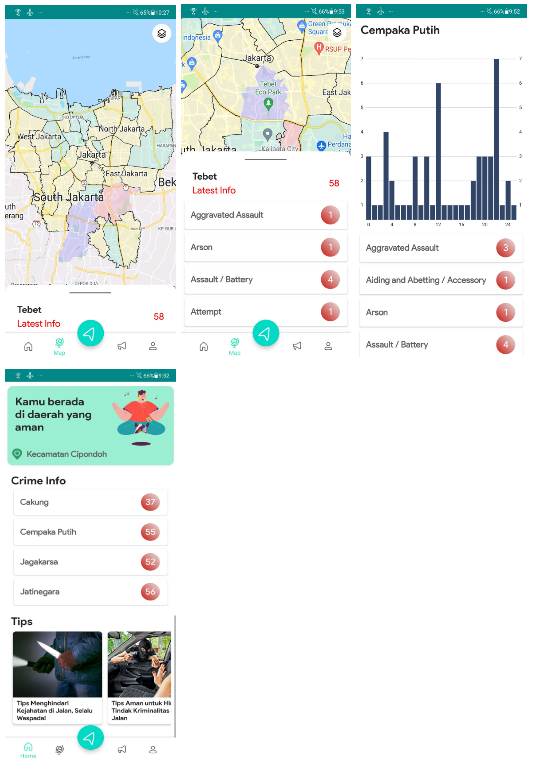
\includegraphics[width=\textwidth]{chapters/images/stats.png}
    \caption{\textit{Area statistic feature (dari kiri ke kanan) chloropleth layer, info panel, statistic drill down, overview}}
    \label{fig:gambar8.1}
\end{figure}

\begin{figure}
    \centering
    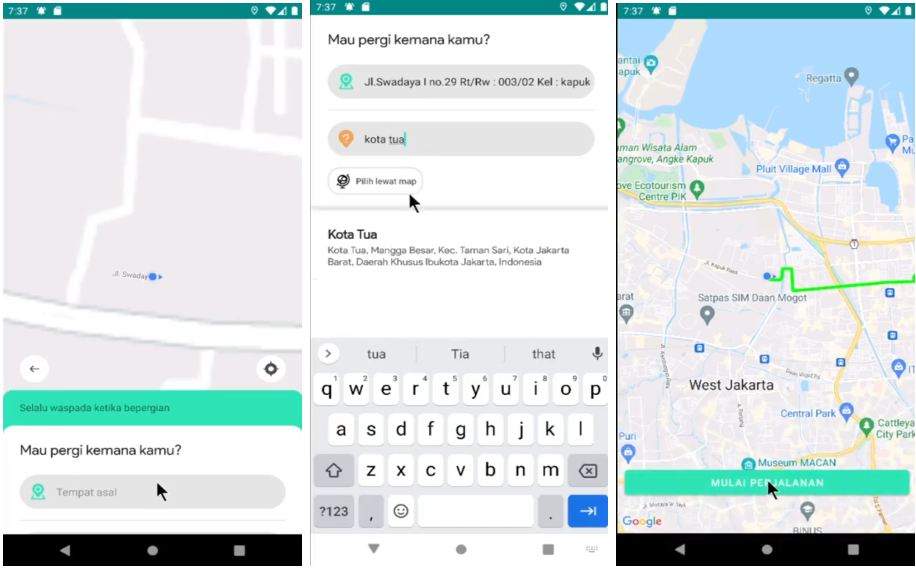
\includegraphics[width=\textwidth]{chapters/images/route-sys.png}
    \caption{\textit{Routing system in the work}}
    \label{fig:gambar8.2}
\end{figure}

\begin{figure}
    \centering
    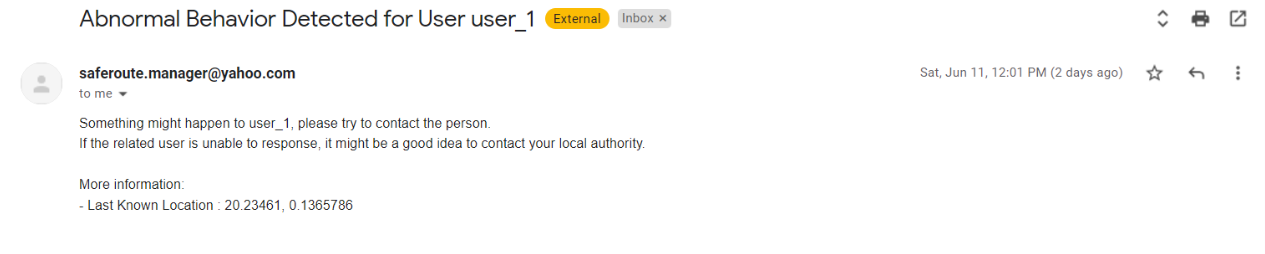
\includegraphics[width=\textwidth]{chapters/images/habit-tracker.png}
    \caption{\textit{Habit tracker anomaly respond email}}
    \label{fig:gambar8.3}
\end{figure}